\chapter{Problématique Réseau et SDN}
\label{chap-1}

%\section{Première section}\label{sec-1-1}

%\section{Deuxième section}\label{sec-1-2}

Ce chapitre reprend les problèmes réseaux rencontrés afin de définir les besoins actuels dans le domaine. 
Une liste de requis pour une architecture réseau idéalement adaptée aux applications actuelles est proposée.
%En connaissant les problèmes de l'architecture en place, la question que se pose est : si on repartait de zéro, comment on le ferrait ?

%\section{Pression pour l'expansion de l'architecture réseau }

\section{Ossification d'internet face aux besoins d'expansion}



%"The classic Internet architecture is a victim of its own success. Having succeeded so well at empowering users and encouraging innovation, it has been made obsolete by explosive growth in users, traffic, applications, and threats." The range of problems observed today is not surprising.

%The Internet was created in simpler times, among a small club of cooperating stakeholders. As the Internet becomes part of more and more aspects of society, it will inevitably be subject to more demands from more stakeholders, and be found deficient in more ways

%In the first half of the 2000s, the research climate was dominated by the belief that research is pointless unless its results can be adopted easily within the existing Internet. Attempting to work within this constraint, people realized that the current architecture makes solving some problems impossible.


À vouloir autoriser et même encourager les utilisateurs à innover sur son architecture, internet s'est fait dépasser par son propre succès. La croissance explosive des utilisateurs, du trafic et des applications a apporté toute une série de problèmes, 
%L'internet a été créé à une époque où les choses étaient plus simples, avec peu d'intervenants en coopération. Dès qu'il est devenu partie intégrante en plusieurs aspects de la société, diverses réclamations et défaillances sont apparues, 
tant la saturation des adresses IPv4 disponibles que les menaces aux réseaux locaux privés. 

%One of the main reasons for these security vulnerabilities is that the Internet architecture and its supporting protocols were primarily designed for a benign and trustworthy environment, with little or no consideration for security issues. This assumption is clearly no longer valid for today’s Internet, which connects millions of people, computers, and corporations in a complex web that spans the entire globe.
\par
En réponse à ces questions, des \glspl{middlebox} ont été introduites dans l'architecture, par exemple les \glspl{nat} et les Firewalls, mais avec une contrainte : la complexité. Dans ces systèmes, le logiciel est capable d'atteindre n'importe quel objectif sous réserve de devenir excessivement complexe, fragile, incompréhensible et mal jugé. Parce que les coûts de la complexité ont été négligés lors de l'évolution d'internet, les applications en réseau ont été rendues difficiles à concevoir, à mettre en place et à maintenir. \cite{InternetEvolutionRoleSoftwareEngineeringRealInternet}

Internet est vu aujourd'hui comme une infrastructure critique de la société, tels que le transport et l'électricité.  Cela provoque une résistance face aux tentatives de nouvelles applications en parallèle à celles en mode de production. 
Cette prise de conscience a convaincu la communauté de chercheurs réseau qu'un travail n'est utile que si ses résultats peuvent être facilement adoptés dans l'architecture existante. 
En essayant de travailler avec cette contrainte, les concepteurs ont réalisé que l'architecture courante rend la résolution de certains problèmes impossible. \cite{OpenFlowStanfordOssification} \cite{SurveySDNIntro}

Actuellement internet doit prendre en compte une énorme base d'équipements et de protocoles installée. Avec le système d'adressage IPv4 ce réseau peut interconnecter jusqu'à quatre milliards d'équipements. Capacité dont la limite est déjà atteinte, fait confirmé par le développement du protocole IPv6 qui a été conçu pour permettre d'augmenter l'espace d'adressage par centaines de milliards de fois. \cite{ICANNIPv6Important} 


Les réseaux de communication des données consistent typiquement à des dispositifs utilisateurs finaux, d'hôtes inter-connectés à travers l'infrastructure du réseau. Cette infrastructure est partagée par ces hôtes et elle emploie des éléments de commutation comme switches et routeurs ainsi que des liens de communication pour porter des données entre les hôtes. Les routeurs et les switches sont souvent des systèmes "fermés", avec des limitations et des interfaces de contrôle spécifiques à leurs vendeurs. 
En raison de ces restrictions, il est assez difficile dans cette infrastructure courante de faire évoluer les protocoles et services existants (déployés en production) et encore plus difficile d'en mettre en place des nouveaux.
%Par conséquent, une fois déployés et en production, il est assez difficile dans cette infrastructure courante de faire évoluer les protocoles et services existants et encore plus difficiles d'en mettre en place des nouveaux. 
Internet étant un réseau de réseaux est particulièrement concerné par ce point. \cite{SurveySDNArchi}
%Data communication networks typically consist of end- user devices, or hosts interconnected by the network infras- tructure. This infrastructure is shared by hosts and employs switching elements such as routers and switches as well as communication links to carry data between hosts. Routers and switches are usually “closed” systems, often with limited- and vendor-specific control interfaces. Therefore, once de- ployed and in production, it is quite difficult for current network infrastructure to evolve; in other words, deploying new versions of existing protocols (e.g., IPv6), not to mention deploying completely new protocols and services is an almost insurmountable obstacle in current networks. The Internet, being a network of networks, is no exception.

%illustrer les problèmes, donner un apperçu



%Complexity matters. The trouble with software is that it can do anything, no matter how complex, convoluted, fragile, incomprehensible, and ill-judged. Software engineers understand the cost of such complexity. Because the networking community underestimates the cost of complexity, it pays no attention to one of the most important problems of the current Internet, which is that it is much too difficult to build, deploy, and maintain networked applications.

%From the viewpoint of Internet users and application programmers, there are requirements that sometimes equal or exceed performance, availability, and efficiency in priority. These include ease of use, correctness, predictability, and modularity.

%The routing table in a typical router now has 300,000 entries, and these must be stored in the fastest, most expensive types of memory to maintain routing speed.

On se rend compte que l'adoption de nouvelles idées dans le domaine des réseaux reste complexe.  Finalement, les ingénieurs comptent sur peu de moyens concrets pour tester de nouveaux protocoles réseau dans une configuration assez réaliste pour assurer et distribuer leurs déploiements. Par conséquent, la majorité des nouvelles idées émises dans le cadre de la recherche en "réseaux informatiques" finissent sans essai et sans test. Ce frein à l'évolution face aux besoins d'expansion des utilisateurs actuels confirme la croyance répandue que l'infrastructure réseau "est en phase d'ossification". \cite{OpenFlowStanfordOssification} 

%quantifier enorme.

\section{Management Réseau : Contraignant et Complexe}

%\subsection*{Brain storming *}

%Même dans un réseau LAN de porte moyen,  on compte avec plusieurs équipements qui réalisent des fonctions spécifiques. Ces équipement doivent être configurable un à un donc pour atteindre à un objectif pour le réseau, tous la configuration de chaque équipement doit être orchestrée pour aboutir ce besoin. Il est difficile de mettre un place une configuration centralisée.

%\par Chaque équipement a été conçu pour réaliser une fonctionnalité spécifique. Pour toute correction de bug ou extension de ces fonctions,  il est nécessaire que le vendeur mette en place une mis à jour logiciel tenant en compte les modifications souhaités ou alors il faut acheter un nouveau équipement. 

%\par Difficulté de faire évoluer (lack of scalability or inability to scale) ; Complexité générant une résistance à l'innovation ; Dépendance du vendeur ; politiques inconsistantes

%Even with the help of autonomous and intelligent agents and network management software, the job of a network administrator is important and complicated. They must balance the different network management areas to make sure their system is properly configured and maintained. 

%The Internet was not designed with management in mind, yet the administrators of today’s networks face critical problems of configuration, traffic engineering, routing policy, and failure diagnosis. Their tools for understanding network traf- fic are poor, and their mechanisms for controlling network operations do not offer a predictable relationship between cause and effect.

%Internet routing is beginning to have serious problems of scale. The routing table in a typical router now has 300,000 entries, and these must be stored in the fastest, most expensive types of memory to maintain routing speed.2 There are efforts to move toward a scheme in which a typical routing table has one entry per autonomous system, which points to a router that can route to all the addresses for which that autonomous system is responsible.

%Network configuration and installation requires highly-skilled personnel adept at configuration of many network elements. Where interactions between network nodes (e.g. switches, routers, etc.) are complex, a more systems-based approach encompassing elements of simulation is required. With the current programming interfaces on much of today’s networking equipment, this is difficult to achieve. In addition, operational costs involved in provisioning and managing large, multi-vendor networks covering multiple technologies have been increasing over recent years, whilst the pre- dominant trend in revenue for operations has been decreasing.

%It was noted that network operation and management is a major source of operating costs, and as well a source of failures and disruptions due to operator error. So we can expect major changes in this area, and we can expect this to be a major focus of a future architecture design.


%Perhaps the attributes most critically lacking are those relating to security, including highly resilient and dependable availability, and a trustworthy environment for people (and their computers) to communicate.

%\subsection*{Fin brain storming *}

Cette résistance à l'innovation est contradictoire avec la rapide croissance d'internet qui impose une expansion de l'architecture réseau. 
Le besoin pour des services réseau et pour haut-débit augmente à un taux plus rapide que la disponibilité ou les revenus, comme on peut le visualiser dans la figure \ref{imgPressure}.


\begin{figure}[!h] %on ouvre l'environnement figure
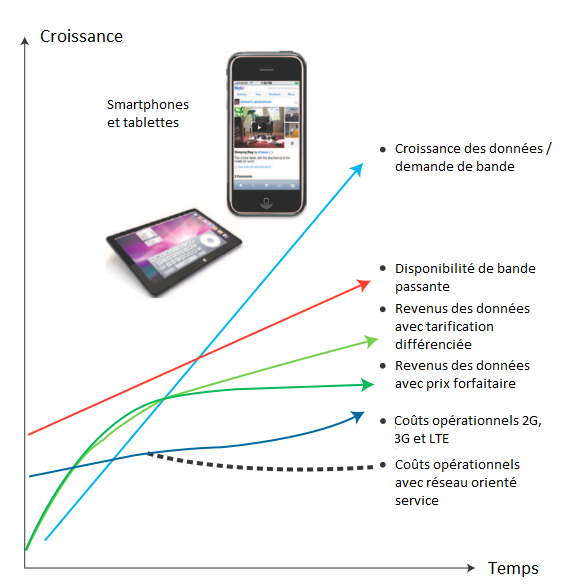
\includegraphics[width=15cm]{images/IncreasingPressureOnNetworkInfra2.png} %ou image.png, .jpeg etc.
\caption{ Pression croissante sur l'infrastructure réseau \cite{IBMManagingGrowingPainsNeed}} %la légende
\label{imgPressure} %l'étiquette pour faire référence à cette image
\end{figure} %on ferme l'environnement figure

Plus une entreprise dépend d'un nombre croissant de dispositifs et gros volumes de données, plus importante est la demande de débit et d'expansion de l'infrastructure. La complexité de cette expansion des réseaux augmente la probabilité des interruptions de service dues à une faille humaine ou autre problème. Ce fait met en évidence l'importance de la disponibilité, la fiabilité, la performance et la sécurité. L'efficacité et la réduction des coûts deviennent cruciales pour aboutir à la mise en échelle de ces besoins, et donc le management doit assumer un rôle primordial dans ce contexte. \cite{IBMManagingGrowingPainsNeed}
 

Malgré l'assistance des agents autonomes et intelligents ainsi que des logiciels pour le management réseau, la mission de l'administrateur réseau reste importante et compliquée. Il doit équilibrer les différentes tâches du management pour assurer que le \gls{si} soit proprement configuré et maintenu. \cite{CentralIssuesNetworkManagementConclusion}

La configuration et l'installation du réseau exigent des techniciens experts hautement qualifiés sur plusieurs éléments le composant. Les interactions entre les nœuds du réseau (switches, routeurs etc.) sont complexes, ce qui oblige à une approche système englobant la simulation. Cette tâche est difficile d'atteindre avec l'interface de programmation des équipements réseau d'aujourd'hui. De plus, les coûts opérationnels pour l'approvisionnement et le management de réseaux larges et multi-vendeurs  couvrant plusieurs technologies ont augmenté récemment, alors que les revenus diminuent. \cite{ImplementationChallengesForSDN}





% Figure 1: The need for network capabilities and bandwidth is expanding at a faster rate than either bandwidth availability or revenue to grow

%\clearpage

L'architecture réseau n'a pas été conçue pour le management, pourtant les administrateurs des réseaux d'aujourd'hui rencontrent des problèmes critiques de configuration, d'ingénierie du trafic, de politique de routage et de diagnostic de failles. Leurs outils pour l'analyse du trafic sont faibles et leurs mécanismes pour contrôler les opérations réseau ne facilitent pas la prédictibilité entre les relations de cause-effet. On réalise que l'opération du réseau et son management représentent la source la plus importante des coûts opérationnels, de failles et d'interruptions à cause d'erreurs des opérateurs. Un changement dans ce domaine est requis pour le design de l'architecture. \cite{NGSIManagement}


\clearpage

%Yet at the same time, society is daring the Internet to face the following set of challenges:
%Security: The lack of security in the Internet is worrisome to ev- eryone including users, application developers, and network and service operators.
%Mobility: Currently, application developers find little support for new mobile applications and services.
%Reliabilityandavailability: ISPsfacethetaskofprovidingaser- vice which meets user expectations of the Internet’s crucial role in both business and private life, in terms of reliability, resilience, and availability, when compared, for example, to the telephone network (five nines1). Furthermore, the service has to be seamless.
%Problem analysis: The toolset for debugging the Internet is lim- ited, e. g., tools for root cause analysis.
%Scalability: Questions remain regarding the scalability of some parts of the current Internet architecture, e.g., the routing system.
%Quality of Service: It is still unclear how and where to integrate different levels of quality of service into the architecture.
%Economics: Besides these more technical questions, there is also the question of how network and service operators can con- tinue to make a profit.



%A new network model is required to support this.
\section{Un nouveau modèle réseau pour supporter ces évolutions}
%\section{Clean-slate Internet}

%While the overall architecture is an undeniable success, the state of the networking industry and the nature of networking infrastructure is a less inspiring story. It is widely agreed that current networks are too expensive, too complicated to manage, too prone to vendor-lockin, and too hard to change. Moreover, this unfortunate state-of-affairs has remained true for well over a decade. Thus, while much of the research community has been focusing on “clean-slate” designs of the overall Internet architecture, a more pressing set of problems remain in the design of the underlying network infrastructure. That is, in addition to worrying about the global Internet protocols, the research community should also devote effort to how one could improve the infrastructure over which these protocols are deployed.

Même si globalement l'architecture réseau d'internet est un succès incontestable, l'état de l'industrie réseau et l'essence de son infrastructure sont moins inspirants. Il est généralement admis que les réseaux courants sont excessivement chers, compliqués à gérer, sujets aux blocages des fournisseurs et difficiles à faire évoluer; de plus, cet état a duré plus d'une décennie. \cite{fabricIntro}



En résumé, l'infrastructure réseau est confrontée actuellement aux challenges suivants :
\begin{itemize}
\item La sécurité : le manque de sécurité est assez inquiétant à tous les niveaux : utilisateurs, développeurs, opérateurs de services. Il manque un point de concentration des flux pour les traitements \gls{ids} et \gls{ips}.
\item La mobilité : il existe très peu de supports pour les applications et services mobiles.
\item La fiabilité et la disponibilité : le nouvel usage de l'internet exige une plus haute fiabilité et une plus haute disponibilité.
\item L'analyse de problèmes : les outils pour déboguer les failles réseau sont assez limités.

%• Simple: The hardware should be inexpensive to build and operate.
%• Vendor-neutral: Users should be able to easily switch between hardware vendors without forklift upgrades.
%• Future-proof: The hardware should, as much as possible, accommodate future innovation, so users need not upgrade their hardware unnecessarily.

\item Le hardware : la simplicité d'opération et l'indépendance des fabricants sont requises.

\item L'évolution : certaines parties de l'architecture courante semblent être saturées, comme le système de routage.
\item La qualité de service : le moyen d'intégrer différents niveaux de \gls{qos} reste toujours incertain.
\item L'économique : outre toutes les questions techniques, il reste aussi la question pour les opérateurs de pouvoir continuer à tirer profit.
\end{itemize}
\cite{InernetCleanSlateDesignIntro}

%In the past 30 years the Internet has been very successful using an incremental approach. However due to its success, the commu- nity has now reached a point where people are unwilling or unable to experiment on the current architecture. Therefore, it might be time to explore a clean-slate approach
L'infrastructure réseau actuelle ne satisfait à aucun de ces objectifs. \cite{fabricIntro}  Dans les dernières 30 années, internet a progressé en utilisant une approche incrémentielle pour répondre aux divers challenges rencontrés. Cependant, ce succès a récemment conduit la communauté à un point où les personnes sont peu disposées ou incapables d'innover sur cette architecture. Pour cette raison, il est peut être le moment d'explorer une nouvelle approche. \cite{InernetCleanSlateDesignApproach}

%Re-partir de zéro. En le faisant, quels sont les caractéristique de l'architecture ?

%blabla...
%Today’s networking infrastructure does not satisfy any of these goals, which is the cause of significant pain for network operators. In fact, in terms of impact on user experience, the inadequacies in these infrastructural aspects are probably more problematic than the Internet’s architectural deficiencies.

Les chercheurs travaillent sur la proposition de cette nouvelle approche pour répondre aux divers challenges rencontrés actuellement. 
%Cette nouvelle architecture à concevoir dans l'infrastructure existante. 
Cette approche doit proposer la conception d'une nouvelle architecture qui permettra à internet et aux réseaux en général de continuer à évoluer et supporter les applications qui répondent aux nouveaux besoins des utilisateurs. 
Basé sur diverses propositions qui émergent depuis quelques années d'études et recherches, \gls{sdn} semble avoir été choisi par la communauté en s'appuyant sur le support des grands leaders du marché.  \cite{SurveySDNIntro}


%\section{Les requis d'un réseau idéalement adapté aux besoins courants}